% Background observer-scale diagnostics — full preprint only.
% Included by paper_full_preprint.tex; not included in the journal submission (paper.tex).
\section{Background Observer-Scale Diagnostics}
\label{app:background}

The main text establishes the embedded-isolate temporal response using the
16-condition GoL/HighLife battery described in Section~\ref{sec:protocol}.
For lineage and context, this appendix records earlier observer-scale
diagnostics from the same research program.
These diagnostics show \emph{why} a target-indexed description analysis
was a natural next step: fine and coarse observers disagree systematically,
and different targets are optimally predicted at different descriptive scales.
\textbf{These figures are background diagnostics only; they are not
load-bearing evidence for the response estimates in the main text.}

\begin{figure*}[t]
  \centering
  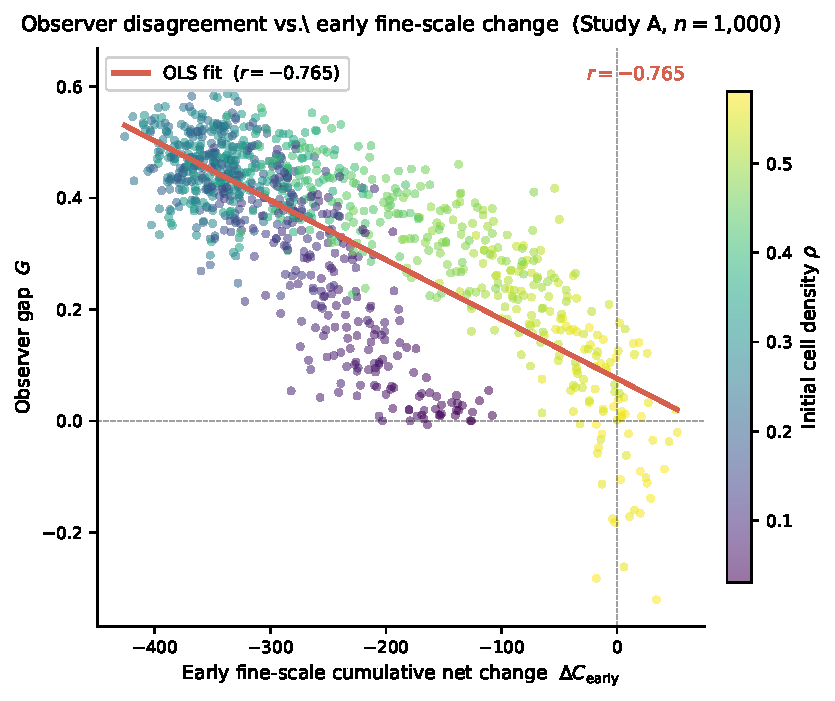
\includegraphics[width=0.82\linewidth]{figures/figE1_disagreement_scatter.pdf}
  \caption{\textbf{E1 --- Observer disagreement scatter (Study A, $n=1{,}000$).}
    Each point is one simulated GoL world.
    $x$-axis: early fine-scale cumulative net component change $\Delta C_{\rm early}$;
    $y$-axis: observer gap $G$ (fine minus coarse observer agreement);
    colour: initial cell density $\rho$.
    The regression line gives $r=-0.765$ ($p \ll 10^{-100}$); partial $r$
    controlling for density $= -0.848$.
    Worlds where fine-scale structure degrades early tend to produce larger
    observer disagreement.
    \textit{Background diagnostic only; not load-bearing for the
    response estimates in the main text.}}
  \label{fig:E1}
\end{figure*}

\begin{figure*}[t]
  \centering
  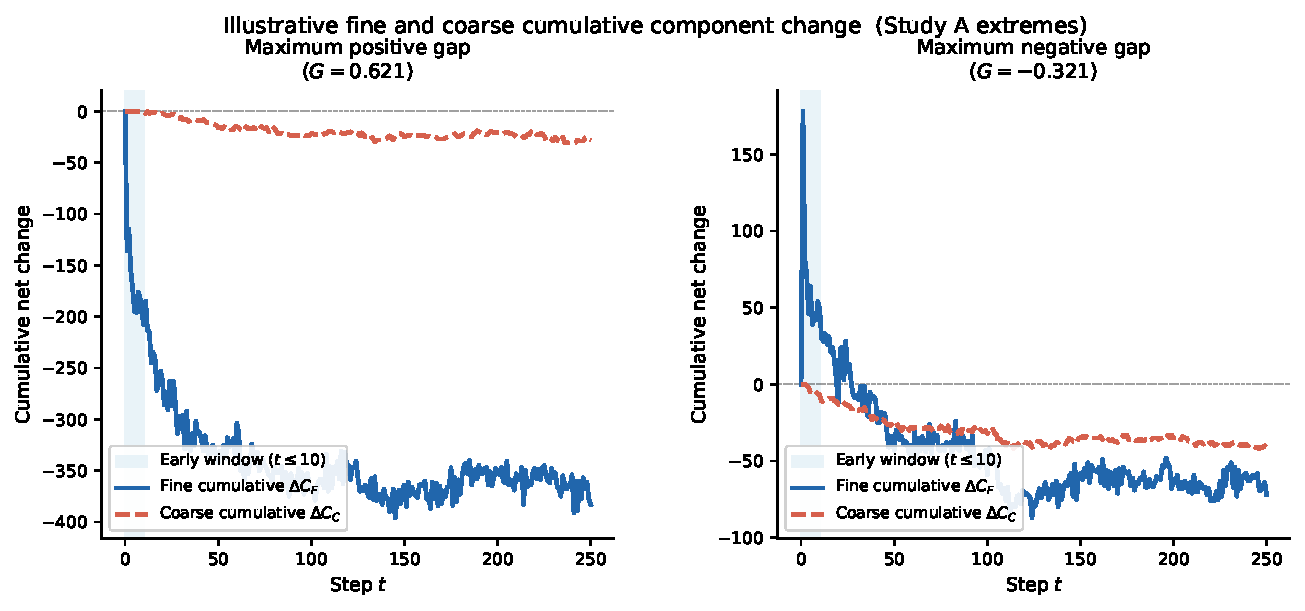
\includegraphics[width=0.95\linewidth]{figures/figE2_trajectories.pdf}
  \caption{\textbf{E2 --- Illustrative fine and coarse observer trajectories (Study A extremes).}
    Left: the world with the maximum positive observer gap ($G=+0.621$).
    Right: the world with the maximum negative gap ($G=-0.321$).
    Blue solid: fine-scale cumulative net component change $\Delta C_F(t)$.
    Orange dashed: coarse-scale cumulative net change $\Delta C_C(t)$.
    Shaded region: early window ($t \leq 10$) whose summary statistic $\Delta C_{\rm early}$
    is used in Figure~\ref{fig:E1}.
    These are selected extreme cases, not representative samples.
    \textit{Background diagnostic only; not load-bearing for the
    response estimates in the main text.}}
  \label{fig:E2}
\end{figure*}

\begin{figure}[t]
  \centering
  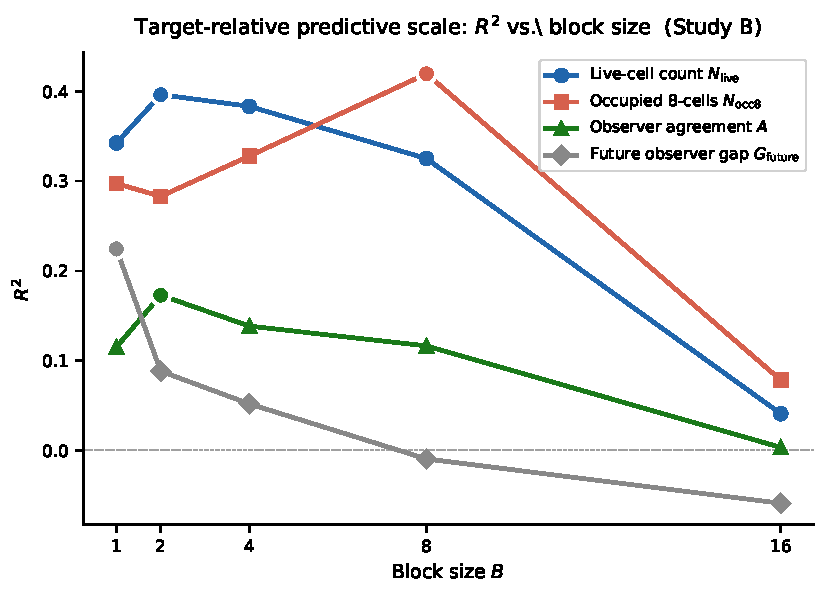
\includegraphics[width=0.85\linewidth]{figures/figE3_scale_R2.pdf}
  \caption{\textbf{E3 --- Target-relative predictive scale (Study B).}
    $R^2$ of a block-aggregated feature predictor as a function of
    block size $B$, separately for four prediction targets.
    $N_{\rm live}$ peaks at $B=2$; $N_{\rm occ8}$ peaks at $B=8$;
    future observer gap $G_{\rm future}$ peaks at $B=1$ and falls steeply;
    observer agreement $A$ is broadly flat then drops.
    Different targets favour different descriptive scales, motivating
    the target-specific framing of the main-text analysis.
    \textit{Background diagnostic only; not load-bearing for the
    response estimates in the main text.}}
  \label{fig:E3}
\end{figure}

\begin{figure}[t]
  \centering
  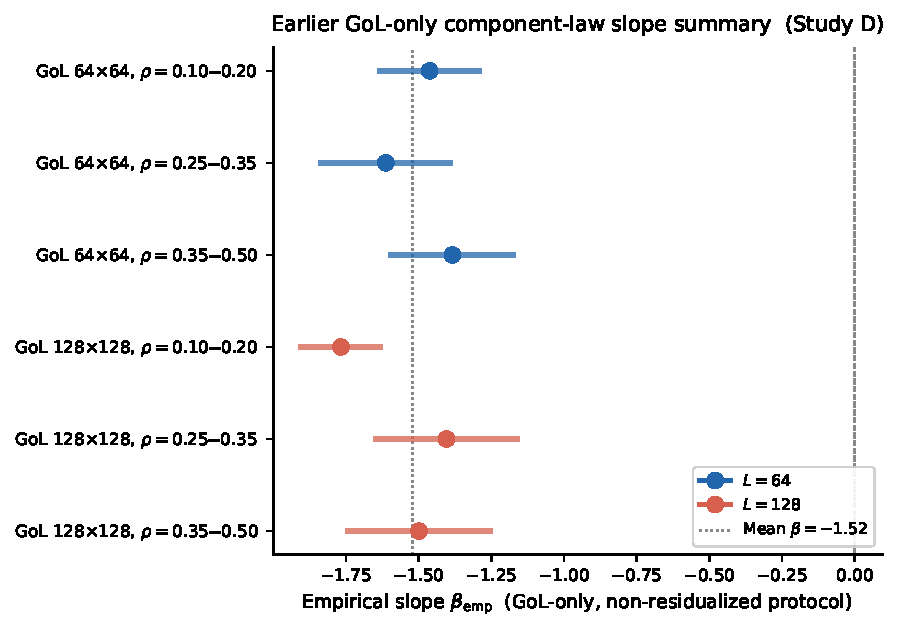
\includegraphics[width=0.88\linewidth]{figures/figE4_old_slopes.pdf}
  \caption{\textbf{E4 --- Earlier GoL-only component-response slope summary (Study D).}
    Empirical slopes $\beta_{\rm emp}$ with 95\% CI for six GoL conditions
    (two grid sizes, three density bands) under an earlier, non-residualized
    regression protocol.
    Mean $\beta \approx -1.52$.
    \textbf{This coefficient is not directly comparable to the residualized
    slopes $\beta_{\rm iso} \approx -0.70$ in the main text:}
    the two studies use different targets, different residualization,
    and different simulation batteries.
    This figure is included as historical lineage only.
    \textit{Background diagnostic only; not load-bearing for the
    response estimates in the main text.}}
  \label{fig:E4}
\end{figure}
